%%%%%%%%%%%%%%%%%%%%%%%%%%%%%%%%%%%%%%%%%%%%%%%%%%%%%%%%%%%%%%%%%%%%%%%%%%%%%%%%
%%                                                                
%%      SWSC LaTeX class for Journal of Space Weather and Space Climate
%%      
%%                                      (c) Springer-Verlag HD
%%                                      revised by EDP Sciences
%%                                      further revised by J. Watermann 
%%
%%%%%%%%%%%%%%%%%%%%%%%%%%%%%%%%%%%%%%%%%%%%%%%%%%%%%%%%%%%%%%%%%%%%%%%%%%%%%%%%
%%
%%      This demonstration file was derived from aa.dem
%%  
%%      AA vers. 7.0, LaTeX class for Astronomy & Astrophysics
%%      demonstration file
%%                                                (c) Springer-Verlag HD
%%                                                revised by EDP Sciences
%%
%%%%%%%%%%%%%%%%%%%%%%%%%%%%%%%%%%%%%%%%%%%%%%%%%%%%%%%%%%%%%%%%%%%%%%%%%%%%%%%%
%%
%%      modified for Journal of Space Weather and Space Climate
%%      by Jurgen Watermann, Editorial Advisor to SWSC
%%
%%      01-04-2012
%%      02-04-2012 revision 1
%%      12-07-2012 revision 2
%%      06-12-2012 revision 3 
%%      01-01-2014 revision 4
%%      06-03-2014 revision 4.1
%%
%%%%%%%%%%%%%%%%%%%%%%%%%%%%%%%%%%%%%%%%%%%%%%%%%%%%%%%%%%%%%%%%%%%%%%%%%%%%%%%%
%%
%%      The two sub-figures referenced in this template are of eps and png type,
%%      respectively, in order to demonstrate the usepackages subfigure and
%%      epstopdf and thus create pdf-only output 
%%
%%      If you want to use TexLive or MikTex together with a bibtex bibliography 
%%      file you may run Latex2e from the command line 
%%          pdflatex -shell-escape swsc.tex
%%          bibtex swsc (do not include an extension such as .tex or .bib)
%%          pdflatex -shell-escape swsc.tex
%%          pdflatex -shell-escape swsc.tex
%%
%%      A double call to pdflatex after calling bibtex is necessary in order to
%%      set citations and references correctly and insure that foreward/backward  
%%      linkage (backref option) is properly applied
%%      If you use MikTex you may need to make a triple call to pdflatex
%%
%%      If you are using TexLive or MikTex but not a bibtex type of bibliography
%%      you may simply run Latex2e twice from the command line 
%%          pdflatex -shell-escape swsc.tex
%%          pdflatex -shell-escape swsc.tex
%%
%%%%%%%%%%%%%%%%%%%%%%%%%%%%%%%%%%%%%%%%%%%%%%%%%%%%%%%%%%%%%%%%%%%%%%%%%%%%%%%%
%%
%%   single column 12-point version for review
%%

%%  with traditional abstract
\documentclass[referee,a4paper,12pt,traditabstract]{swsc} 

%%  with structured abstract 
%\documentclass[referee,a4paper,12pt,structabstract]{swsc} 

\usepackage{graphicx}
\usepackage{txfonts}
\usepackage{subfigure}
\usepackage{epstopdf}
\usepackage{lineno}
\usepackage[authoryear,round]{natbib}
\usepackage[backref]{hyperref}
\usepackage{url}
\usepackage[inline]{enumitem}
\usepackage{verbatim}
%%    This version assumes using bibtex with the swsc bibliography style file
\bibliographystyle{swsc.bst}

\hypersetup{colorlinks=true,citecolor=cyan,urlcolor=cyan,linkcolor=blue}

%%%%%%%%%%%%%%%%%%%%%%%%%%%%%%%%%%%%%%%%%%%%%%%%%%%%%%%%%%%%%%%%%%%%%%%%%%%%%%%%

\begin{document}

\begin{linenumbers}

   \title{Gaussian Processes Autoregressive Models for the Disturbance Storm Time Index}

   \subtitle{Attaining performance over and above persistence behavior}
   
   \titlerunning{Gaussian Process $D_{st}$ models}

   \authorrunning{Chandorkar and Camporeale}

   \author{M. Chandorkar
          \inst{1}
          \and
          E. Camporeale\inst{1}
          }

   \institute{Centrum Wiskunde Informatica (CWI), Amsterdam,
              1098XG Amsterdam\\
              \email{\href{mailto:m.h.chandorkar@cwi.nl}{m.h.chandorkar@cwi.nl} \href{mailto:e.camporeale@cwi.nl}{e.camporeale@cwi.nl}} 
             }

%%   \date{Received September 15, 1996; accepted March 16, 1997}

  % \abstract{}{}{}{}{}        %% uncomment if structured abstract is desired
 %% 5 {} token are mandatory
 
   %% replace by pair of curly brackets, {}, if structured abstract is selected
   
   
   \abstract{
    We aim to improve the state of the art of \emph{One Step Ahead}(OSA) prediction of the $D_{st}$ geomagnetic activity index. In the domain of OSA prediction, it is well known that $D_{st}(t)$ values correlate strongly with values one hour in the past (i.e. $D_{st}(t-1)$). While a number of forecasting models have been proposed and compared, none of them have been compared with the \emph{Persistence} model to quantify their performance improvements above this most trivial of predictors. In this study we train Gaussian Process regression models for One Step Ahead (OSE) prediction of the Disturbance Storm Time ($D_{st}$) geomagnetic index. We propose three variants of the Gaussian Process model.
    \begin{enumerate*}
      \item Gaussian Process Auto regressive (GP-AR) 
      \item Gaussian Process Auto regressive with eXogenous inputs (GP-ARX). 
    \end{enumerate*}
    We compare the performance of these models with the current state of the art in one step ahead $D_{st}$ prediction on a set of 
    63 benchmark storms from 1998-2006. The proposed Gaussian Process models not only outperform the rest but also the \emph{Persistence} model.
    }

   \keywords{Geomagnetic indices --
            $D_{st}$ OSA Prediction --
            Gaussian Processes --
            Machine Learning
            }

   \maketitle
%%
%%________________________________________________________________

\section{Introduction}

The Sun is the principal driver of Space Weather, the steady solar wind and intermittent bursts of hot plasma from its corona (Coronal Mass Ejections \emph{CME}) are the causes of several observed phenomena in the Earths Magnetosphere such as but not limited to \emph{Aurora Borealis}, \emph{Aurora Australis}, \emph{Van Allen Currents}, geomagnetic storms etc.

Although the qualitative bifurcation of these phenomena is well understood and each has been studied in depth, the magnetosphere's dynamics and its associated solar wind driver form a complex nonlinear coupled dynamical system. It is therefore not only instructive but also greatly simplifying to use representative indices to quantify the state of geomagnetic activity.

Geomagnetic indices come in various forms, they may take continuous or discreet values. Their values are often calculated by averaging or combining a number of readings taken by instruments around the Earth. Each geomagnetic index is a proxy for a particular kind of phenomena. Some popular indices are the $K_p$, $D_{st}$ and the AE index.

\begin{comment}
\begin{enumerate}
    \item $K_p$: The Kp-index is a discreet valued global geomagnetic storm index and is based on 3 hour measurements of the K-indices, for a given value, for each of the past days. The K-index itself is a three hour long quasi-logarithmic local index of the geomagnetic activity, relative to a calm day curve for the given location.
    
    \item AE: The Auroral Electrojet Index, AE, is designed to provide a global, quantitative measure of auroral zone magnetic activity produced by enhanced Ionospheric currents flowing below and within the auroral oval.
    
    \item $D_{st}$: A continuous hourly index which measures the weakening of the Earths magnetic field due to ring currents. 
\end{enumerate}
\end{comment}

%Talk about Burton and friends
We focus on prediction of the hourly $D_{st}$ index which is an important problem because $D_{st}$ is a straightforward indicator of geomagnetic storms. More specifically we focus on the \emph{one step ahead} (OSA) prediction of $D_{st}$ because it is the first step towards building long term predictions of geomagnetic response of the Earth to changing space weather conditions. 

The $D_{st}$ OSA prediction problem has been the subject of several modeling efforts so far, some of the earliest are by \citet{JGR:JGR10260} who outlined a prediction framework that has been used as a starting point for many $D_{st}$ models. \citet{JGR:JGR10260} model $D_{st}(t)$ a function of time using an \emph{Ordinary Differential Equation} (ODE) which expressed it's rate of change as a combination of two terms: decay and injection $\frac{d D_{st}(t)}{dt} = Q(t) - \frac{D_{st}(t)}{\tau}$. 

The \citet{JGR:JGR10260} model has proven to be very influential in the Space Weather research effort and many subsequent works like \citet{Wang:Dst}, \citet{JGRA:JGRA14856} modified the proposed ODE by proposing expressions for the injection term $Q(t)$. More recently \citet{Ballatore2014} have tried to generate empirical estimates for the injection and decay terms in Burton's equation.

%Talk about NARMAX Dst
Among the other major empirical models used to predict $D_{st}$ has been the \emph{Nonlinear Auto-Regessive Moving Average with eXogenous inputs} (NARMAX) methodology developed in \citet{doi:10.1080/00207178908559767}, \citet{GRL:GRL13494}, \citet{GRL:GRL20944}, \citet{JGRA:JGRA18657}, \citet{balikhin:narmax}, \citet{JGRA:JGRA20661} and \citet{JGRA:JGRA50192}. The NARMAX methodology builds models by constructing polynomial expansions of inputs and determines the best combinations or monomials to include in the refined model using the \emph{error reduction ratio} (ERR) criterion. The parameters of the NARMAX OLS-ERR model are calculated using the standard \emph{ordinary least squares} (OLS) method hence these methods are also denoted by the acronym NARMAX OLS-ERR. The reader may refer to \citet{billings2013nonlinear} for a detailed exposition of the NARMAX methodology.

%Talk about neural networks
\emph{Neural Networks} have been a popular choice for building predictive models and researchers employed the standard \emph{feed forward} and the more specialized \emph{recurrent} architectures. \citet{Lund} proposed an \emph{Elman} recurrent network architecture called Lund $D_{st}$, which used the solar wind, \emph{interplanetary magnetic field} (IMF) and historical $D_{st}$ data. \citet{SWE:SWE286} originally proposed a \emph{feed forward} network for predicting the $K_p$ index which used the \emph{Boyle coupling function} (\citet{boyle1997empirical}), in \citet{SWE:SWE286} the same architecture is adapted for prediction of $D_{st}$, which is popularly known as the Rice $D_{st}$ model. \citet{pallocchia:hal-00318011} proposed a \emph{neural network} model called EDDA to predict $D_{st}$ using only the IMF data.

%Talk about comparison papers, number of storms covered and Persistence
In light of the extensive list of modeling techniques employed for prediction of geomagnetic indices and in particular $D_{st}$, model comparison and evaluation becomes a crucial direction in advancing the research domain. \citet{Rastatter2013} compare several physics based (convection, kinetic and magneto hydrodynamic) and empirical prediction models such as Narmax, Rice $D_{st}$ on 4 storm events which occurred between 2001 and 2006. \citet{Amata2008} compares the EDDA and the Lund $D_{st}$ models over the 2003-2005 period. But the most extensive model comparison in terms of storm events was conducted in \citet{Ji2012} which compared seven $D_{st}$ models (see table \ref{table:DstModels}) on a list of 63 geomagnetic storm events of varying intensities which occurred between 1998 and 2006. 

%Vision
In $D_{st}$ prediction a seemingly trivial yet highly informative prediction method known as the \emph{Persistence} model has been largely ignored in its crucial role in model evaluation. The \emph{Persistence} model is stated simply as using the previous value of $D_{st}$ as the prediction for the next time step ($\hat{D_{st}}(t) = D_{st}(t-1)$). Due to high auto correlation between $D_{st}(t)$ and $D_{st}(t-1)$ in the Omni data, the \emph{Persistence} model gives excellent predictive performance despite its apparent lack of sophistication. In essence it is a trivial hypothesis and hence must always be used as a base line to compare the performance of any proposed $D_{st}$ algorithm. Therefore in the context of OSA prediction, a model must outperform the \emph{Persistence} model in order to be a viable candidate for advancing the science of space weather prediction.

%Assertion
It is with the above observation in mind, we propose \emph{Gaussian Process} models for OSA prediction of $D_{st}$. We use the results of \citet{Ji2012} as a starting point and compare our proposed models with the methods outlined in the same paper while using the performance of the \emph{Persistence} model as a litmus test. 

% Talk about Gaussian Process
We use the hourly resolution Omni data set (see \cite{OmniPaper}) as extracted from NASA/GSFC's OMNI data set through OMNIWeb. The rest of the paper is organized as follows. Section \ref{sec:method} gives an introduction to the \emph{Gaussian Process} methodology for regression and the various issues surrounding their application. In section \ref{sec:osa} two different \emph{Gaussian Process} auto-regressive models are proposed and subsequently in sections \ref{sec:exp} and \ref{sec:res}, bench marked against the \emph{Persistence} $D_{st}$ model as well as other models outlined in \citet{Ji2012}.

  
\section{Methodology: Gaussian Process} \label{sec:method}

A \emph{Gaussian Process} is a stochastic process $f(\mathbf{x}), \ \mathbf{x} \in \mathbb{R}^d$ whose finite dimensional distributions over a set of points $\mathbf{x}_1, \cdots, \mathbf{x}_n$ are multivariate Gaussian. Formally this is expressed as.

\begin{eqnarray}
 \mathbf{f} & = & \left( \begin{array}{c} f(\mathbf{x}_1) \\ f(\mathbf{x}_2) \\ \vdots \\ f(\mathbf{x}_n) \end{array} \right) \\
 \vspace{2\baselineskip}
 \mathbf{f} | \mathbf{x}_1, \cdots, \mathbf{x}_n & \sim & \mathcal{N}\left( \mathbf{\mu}, \mathbf{\Lambda} \right)  \\
 \vspace{2\baselineskip}
 p( \mathbf{f} \ | \ \mathbf{x}_1, \cdots, \mathbf{x}_n) & = & \frac{1}{(2\pi)^{n/2} det(\mathbf{\Lambda})^{1/2}} exp \left(-\frac{1}{2} (\mathbf{f} - \mathbf{\mu})^T \mathbf{\Lambda}^{-1} (\mathbf{f} - \mathbf{\mu}) \right) \label{eq:sto}
\end{eqnarray}

From equation \ref{eq:sto}, one can observe that in order to uniquely define the distribution of the process, it is required to specify the mean vector $\mathbf{\mu}$ and the covariance matrix $\mathbf{\Lambda}$. For this probability density to be valid, there is a further requirements imposed on $\mathbf{\Lambda}$: 

\begin{enumerate}
      \item Symmetry: $\mathbf{\Lambda}_{ij} = \mathbf{\Lambda}_{ij} \ \forall i,j \in {1, \cdots, n} $ 
      \item Positive Semi-definiteness: $\mathbf{y}^T \mathbf{\Lambda} \mathbf{y} \geq 0 \ \forall \mathbf{y} \in \mathbb{R}^n$  
\end{enumerate}

Inspecting the individual elements of $\mathbf{\mu}$ and $\mathbf{\Lambda}$, we realise that they take the following form.

\begin{eqnarray}
      \mu_i & = & \mathbb{E}[f(\mathbf{x}_i)] := m(\mathbf{x}_i) \\
      \Lambda_{ij} & = & \mathbb{E}[(f(\mathbf{x}_i) - \mu_i)(f(\mathbf{x}_j) - \mu_j)] := K(\mathbf{x}_i, \mathbf{x}_j)
\end{eqnarray}

Here $\mathbb{E}$ denotes the expectation (average). The elements of $\mathbf{\mu}$ and $\mathbf{\Lambda}$ are expressed as functions $m(\mathbf{x}_i)$ and $K(\mathbf{x}_i, \mathbf{x}_j)$ of the inputs $\mathbf{x}_i,\ \mathbf{x}_j$. Specifying the functions $m(\mathbf{x})$ and $K(\mathbf{x}, \mathbf{x}')$ completely specifies each element of $\mathbf{\mu}$ and $\mathbf{\Lambda}$ and subsequently the finite dimensional distribution of $\mathbf{f} | \mathbf{x}_1, \cdots, \mathbf{x}_n $. In machine learning literature \emph{Gaussian Processes} are represented using the following notation.

\begin{equation}
    f(\mathbf{x}) \sim \mathcal{GP}(m(\mathbf{x}), K(\mathbf{x}, \mathbf{x}'))
\end{equation}

In most practical applications of \emph{Gaussian Processes} the mean function is often defined as $m(\mathbf{x}) = 0$, which is not unreasonable if the data is standardized to have zero mean. The central design issue now becomes choice of the function $K(\mathbf{x}, \mathbf{x}')$. The same constraints that apply to $\mathbf{\Lambda}$ also apply to the function $K(.,.)$. In machine learning, these symmetric positive definite functions of two variables are known as \emph{kernels}. Kernel based methods are applied extensively in data analysis i.e. regression, clustering, classification, density estimation (see \citet{Scholkopf:2001:LKS:559923}, \citet{hofmann2008}).

\emph{Gaussian Processes} first appeared in machine learning research in \citet{Neal:1996:BLN:525544}, as the limiting case of Bayesian inference performed on neural networks with infinitely many neurons in the hidden layers. Although their inception in the machine learning community is recent, their origins can be traced back to the geo-statistics research community where they are known as \emph{Kriging} methods (\citet{krige1951statistical}). In pure mathematics area \emph{Gaussian Processes} have been studied extensively and their existence was first proven by Kolmogorov's extension theorem (\citet{tao2011introduction}). The reader is requested to refer to \cite{Rasmussen:2005:GPM:1162254} for an in depth treatment of Gaussian Processes in machine learning.

\subsection{Gaussian Process Regression: Formulation}

\begin{eqnarray}
  \mathbf{X} & = & \left( \begin{array}{c} \mathbf{x}^{T}_1 \\ \mathbf{x}^{T}_2 \\ \vdots \\ \mathbf{x}^{T}_n \end{array} \right)_{n \times d} \label{eq:feat} \\
  \vspace{2\baselineskip}
  \mathbf{y} & = & \left( \begin{array}{c} y_1 \\ y_2 \\ \vdots \\ y_N \end{array} \right) _{n \times 1} \label{eq:labels}
\end{eqnarray}

We start with a set of labeled data points $ {(\mathbf{x}_i, y_i): \forall i \in 1 \cdots N, \ \mathbf{x}_i \in \mathbb{R}^d \ y_i \in \mathbb{R}} $ condensed into a data matrix $\mathbf{X}$ and response vector $\mathbf{y}$ in equations \ref{eq:feat} and \ref{eq:labels}. The values $y_i$ are assumed to be measurements of an unknown function $f(\mathbf{x}_i)$ corrupted by an independent and identically distributed zero mean Gaussian noise. The \emph{Gaussian Process} regression framework is the defined by the following components.

\begin{eqnarray}
      y & = & f(\mathbf{x}) + \epsilon  \\
      \epsilon & \sim & \mathcal{N}(0, \sigma^2) \\
      f(\mathbf{x}) & \sim & \mathcal{GP}(m(\mathbf{x}), K(\mathbf{x},\mathbf{x}')) 
\end{eqnarray}


\subsection{Inference and Predictions}

Our aim is to generate infer the function $f(\mathbf{x})$ from the noisy training data and generate predictions $f(\mathbf{x}^{*}_i)$ for a set of test points $ {\mathbf{x}^{*}_i : \forall i \in 1, \cdots, m} $. We start from equation \ref{eq:sto} and use it to construct the distribution of $f(\mathbf{x})$ over the training and test points, how ever since we have noisy measurements of $f$ over the training data, we add the noise variance $\sigma^2$ to the variance of $f$ as shown in \ref{eq:dist}.

\begin{eqnarray}
    \mathbf{X}_* & = & \left( \begin{array}{c} (\mathbf{x}^{*}_1)^T \\ (\mathbf{x}^{*}_2)^T \\ \vdots \\ (\mathbf{x}^{*}_m)^T \end{array} \right)_{m \times d} \\
    \mathbf{f}_* & = & \left( \begin{array}{c} f(\mathbf{x^{*}_1}) \\ f(\mathbf{x^{*}_2}) \\ \vdots \\ f(\mathbf{x^{*}_m}) \end{array} \right)_{m \times 1} \\
     \vspace{4\baselineskip}
    \left( \begin{array}{c} \mathbf{y} \\ \mathbf{f_*} \end{array} \right) | \ \ \mathbf{X}, \mathbf{X}_* & \sim & 
    \mathcal{N}\left(\mathbf{0}, \left[ \begin{array}{cc} \mathbf{K} + \sigma^{2} \mathbf{I} & \mathbf{K}_{*} \\ \mathbf{K}_{*}^T & \mathbf{K}_{**} \end{array} \right ] \right) \label{eq:dist}
\end{eqnarray}

In equation \ref{eq:dist} the block matrix components of the $n+m \times n+m$ covariance matrix have the following structure.

\begin{enumerate}
      \item $\mathbf{I}$: The $n \times n$ identity matrix.
      \item $\mathbf{K} = [K(\mathbf{x}_i, \mathbf{x}_j)], \ i,j \in 1,\cdots,n$ : Kernel matrix constructed from all couples of the training data.
      \item $\mathbf{K}_{*} = [K(\mathbf{x}_i, \mathbf{x}^{*}_j)], \ i \in 1,\cdots,n ; j \in 1,\cdots,m$ : Cross kernel matrix constructed from all couples between training and test data points.
      \item $\mathbf{K}_{**} = [K(\mathbf{x}^{*}_i, \mathbf{x}^{*}_j)], \ i,j \in 1,\cdots,m$: Kernel matrix constructed from all couples of the test data.
\end{enumerate}

With the multivariate normal distribution defined in equation \ref{eq:dist}, probabilistic predictions $f_*$ can be generated by constructing the conditional distribution $\mathbf{f_*}|\mathbf{X},\mathbf{y},\mathbf{X_*}$, since the original distribution of $\left( \begin{array}{c} \mathbf{y} \\ \mathbf{f_*} \end{array} \right) | \ \ \mathbf{X}, \mathbf{X}_*$ is a multivariate Gaussian, conditioning on a subset of elements $\mathbf{y}$ yields another Gaussian distribution with mean and covariance given below \ref{eq:posterior}.

\begin{eqnarray}
    \mathbf{f_*}|\mathbf{X},\mathbf{y},\mathbf{X_*} & \sim & \mathcal{N}(\mathbf{\bar{f}_*}, \Sigma_*)  \label{eq:posterior} \\
    \mathbf{\bar{f}_*} & = & \mathbf{K}^T_{*} [\mathbf{K} + \sigma^{2} \mathbf{I}]^{-1} \mathbf{y} \label{eq:posteriormean} \\
    \Sigma_* & = & \mathbf{K}_{**} - \mathbf{K}^T_{*} \left(\mathbf{K} + \sigma^{2} \mathbf{I}\right)^{-1} \mathbf{K}_{*} \label{eq:posteriorcov}
\end{eqnarray}

The distribution of $\mathbf{f_*}| \mathbf{X},\mathbf{y},\mathbf{X_*}$ is known in Bayesian analysis as the \emph{Posterior Predictive Distribution}. This illustrates a key difference between \emph{Gaussian Processes} and other regression models such as \emph{Neural Networks}, \emph{Linear Models} and \emph{Support Vector Machines}, that a \emph{Gaussian Process} model does not generate point predictions for new data but outputs a predictive distribution for the quantity sought, this allows us to construct error bars on the predictions. This property of Bayesian models such as \emph{Gaussian Processes} makes them suitable for Space Weather forecasting applications. 

\subsection{Kernel Functions}

For the success of a Gaussian Process model an appropriate choice of kernel function is paramount. The symmetry and positive semi-definiteness of \emph{Gaussian Process} kernels implies that they represent inner-products between some basis function representation of the data. This is analogous to a Fourier series decomposition in Physics. The interested reader is suggested to refer to \cite{Berlinet2004}, \citet{Scholkopf:2001:LKS:559923} and \citet{hofmann2008} for a thorough treatment on kernel functions and the rich theory behind them. Some common kernel functions used in machine learning are.

\subsubsection{Radial Basis Function (RBF)}

The RBF kernel is the most commonly used kernel in machine learning, in its core it encodes the idea of \emph{smoothness} because functions drawn from its Hilbert space are infinitely differentiable. The RBF kernel is also an example of a \emph{stationary} kernel i.e. its value depends only on $||\mathbf{x} - \mathbf{y}||$. The quantity $l$ is known as the characteristic \emph{length scale} of this kernel, it is a free parameter (also known as hyper-parameter) which must be determined by the modeller, refer to section \ref{sec:hyp} on how suitable values of kernel hyper-parameters.

\begin{equation}
    K(\mathbf{x}, \mathbf{y}) = \frac{1}{2} exp(-||\mathbf{x} - \mathbf{y}||^2/l^2)
\end{equation}
    
    
\subsubsection{Polynomial}

The polynomial kernel is also a common kernel function employed in research, it has two hyper-parameters the degree $d$ and an intercept $b$. The polynomial kernel formulates the function approximation in terms of polynomial expansions of the input dimensions $\mathbf{x}$, more specifically it considers all monomial combination of the input dimensions up to degree $d$. When $d = 1$ it corresponds to a Bayesian linear regression model. 

\begin{equation}
    K(\mathbf{x}, \mathbf{y}) = (\mathbf{x}^\intercal \mathbf{y} + b)^d 
\end{equation}

In this study, we construct Gaussian Process regression models with polynomial kernels for \emph{one step ahead} prediction of the $D_{st}$ index. 

\subsection{Optimizing Hyper-parameters} \label{sec:hyp}

When fitting \emph{Gaussian Process} models to data, the question to be answered following choice of a kernel function is the assignment of appropriate values to the kernel hyper-parameters and noise level ($\sigma^2$). This is known as the problem of \emph{model selection}.

Common examples of criteria used for \emph{model selection} include data likelihood, cross validation performance scores and validation set performance scores among others. Since model selection criteria are non-convex and non-smooth in general, gradient free approaches are used to find approximate values of local optima.

The simplest way to perform \emph{model selection} is called \emph{grid search} which entails evaluating the above criteria on a fixed grid which is constructed by making a list of values for each hyper-parameter and taking the combinations of all such values. There are more sophisticated methods for \emph{model tuning} such as \emph{coupled simulated annealing} (\citet{Xavier-De-Souza2010}) and \emph{simplex search} (\citet{Nelder1965}) but they are computationally more expensive. 

In this study we employ \emph{grid search} to find the best performing set of hyper-parameter assignments inside a predefined grid of possible hyper-parameter values.


\section{One Step Ahead Prediction} \label{sec:osa}

Below in equations \ref{eq:Dst}, \ref{eq:GPNoise}, \ref{eq:DstGP}, \ref{eq:GPPoly} we outline a \emph{Gaussian Process} formulation for \emph{OSA} prediction of $D_{st}$. A vector of features $x_{t-1}$ is used as input to an unknown function $f(x_{t-1})$ which drawn from a \emph{Gaussian Process} driven by a linear polynomial kernel. 

The features $x_{t-1}$ can be any collection of quantities in the hourly resolution Omni data set. Generally $x_{t-1}$ are time histories of $D_{st}$ or other important variables examples being plasma pressure $p(t)$, solar wind speed $V(t)$, z component of the interplanetary magnetic field $B_z(t)$.

\begin{eqnarray}
    D_{st}(t) & = & f(\mathbf{x}_{t-1}) + \epsilon \label{eq:Dst} \\
    \epsilon & \sim & \mathcal{N}(0, \sigma^2) \label{eq:GPNoise} \\
    f(x_t) & \sim & \mathcal{GP}(m(\mathbf{x}_t), K(\mathbf{x}_t, \mathbf{x}_s)) \label{eq:DstGP} \\
    K(\mathbf{x}, \mathbf{y}) & = & \mathbf{x}^\intercal \mathbf{y} + b \label{eq:GPPoly}
\end{eqnarray}

In \ref{sec:gpar} and \ref{sec:gparx} below we consider two choices for the input features $\mathbf{x}_{t-1}$ leading to two variants of \emph{Gaussian Process} regression for $D_{st}$ time series prediction.

\subsection{Gaussian Process Auto-Regressive (GP-AR)} \label{sec:gpar}

The simplest auto-regressive models for \emph{OSA} prediction of $D_{st}$ are those that use only the history of $D_{st}$ to construct input features for model training. The input features $\mathbf{x}_{t-1}$ at each time step is the history of $D_{st}(t)$ until a time lag of $p$ steps.

\begin{eqnarray*}
    \mathbf{x}_t & = & \left(D_{st}(t), D_{st}(t-1), \cdots , D_{st}(t-p+1)\right)
\end{eqnarray*}

\subsection{Gaussian Process Auto-Regressive with eXogenous inputs (GP-ARX)} \label{sec:gparx}

Auto-regressive models can be improved by including exogenous quantities that can help in improving predictions. It is well known that the solar wind and interplanetary magnetic field are important factors that influence the Earth's geomagnetic state.

Hourly solar wind velocity $V(t)$ and interplanetary magnetic field $B_z(t)$ recorded at the ACE satellite are used as the exogenous inputs of the model, along with the time history of $D_{st}$. In this model we choose distinct time lags $p$ and $p_{ex}$ for auto-regressive and exogenous variables respectively.
    
\begin{eqnarray*}
        & \mathbf{x}_t & = (D_{st}(t), D_{st}(t-1), \cdots , D_{st}(t-p+1), \\
        & \ \ \ \ \ & V(t), V(t-1), \cdots, V(t-p_{ex}+1),\\
        & \ \ \ \ \ & B_{z}(t), B_{z}(t-1), \cdots, B_{z}(t-p_{ex}+1),\\
        & \ \ \ \ \ & V B_{z}(t), V B_{z}(t-1), \cdots, V B_{z}(t-p_{ex}+1))
\end{eqnarray*}

\section{Model Training and Validation}

Before performance bench marks for \emph{OSA} $D_{st}$ prediction are run on the storm events in \cite{Ji2012}, training and model selection of \emph{GP-AR} and \emph{GP-ARX} models on independent data sets must be performed. For this purpose we choose segments 00:00 1 January 2008 - 10:00 11 January 2008 and 00:00 15 November 2014 - 23:00 1 December 2014 for training and model selection respectively.

Model selection of \emph{GP-AR} and \emph{GP-ARX} is performed by grid search methodology and the root mean square error (\emph{RMSE}) on the validation set is used to select the values of the model hyper-parameters. The time lags chosen for \emph{GP-AR} are $p = 6$ while for \emph{GP-ARX} $p=6$, $p_{ex} = 1$ are arrived by experimenting with values starting from one and choosing the value of $p$ yielding best performance on the 63 events in the bench mark.   

\begin{figure}
   \centering
   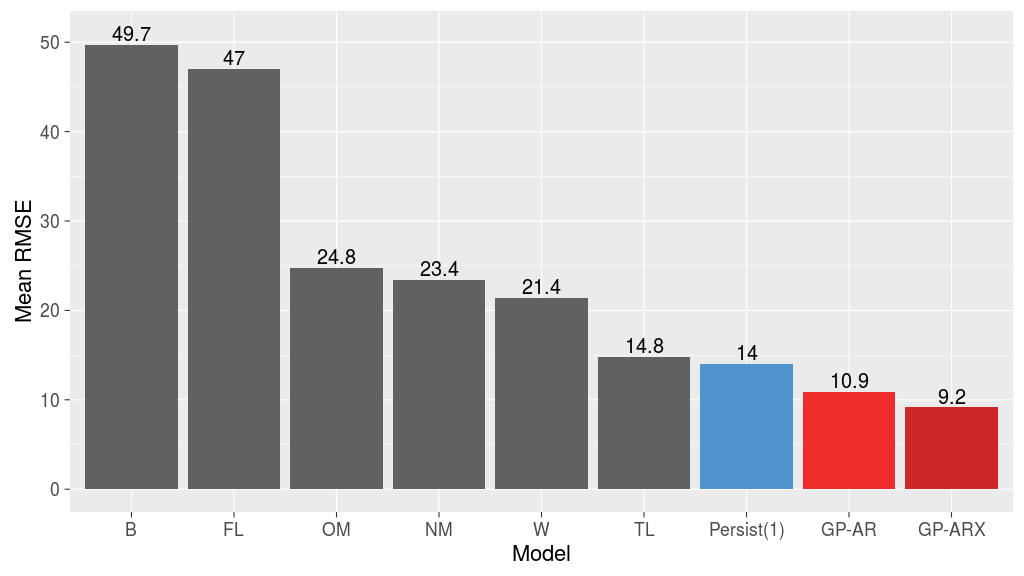
\includegraphics[width=\textwidth]{Compare_RMSE.png}
      \caption{Averaged RMSE}
         \label{fig:rmse}
   \end{figure}

\section{Experiments} \label{sec:exp}

\citet{Ji2012} compare a six OSA $D_{st}$ models in their paper by compiling a list of 63 geomagnetic storm events of varying strengths which occurred from 1998-2006. This serves as an important stepping stone for a systematic comparison of existing and new prediction techniques because performance metrics are averaged over a large number of storm events that occurred over a 8 year period. They compare the averaged performance of these models on four key performance metrics.

\begin{enumerate}
    \item $RMSE$: The root mean square error
    \item $CC$: Correlation coefficient between the predicted and actual value of $D_{st}$
    \item $\Delta Dst_{min}$: The error in prediction of the peak value of $D_{st}$ for a storm event.
    \item $|\Delta t_{peak}|$: The error in predicting the timing of a storm peak, also called \emph{timing error}. 
\end{enumerate}


\begin{figure}
   \centering
   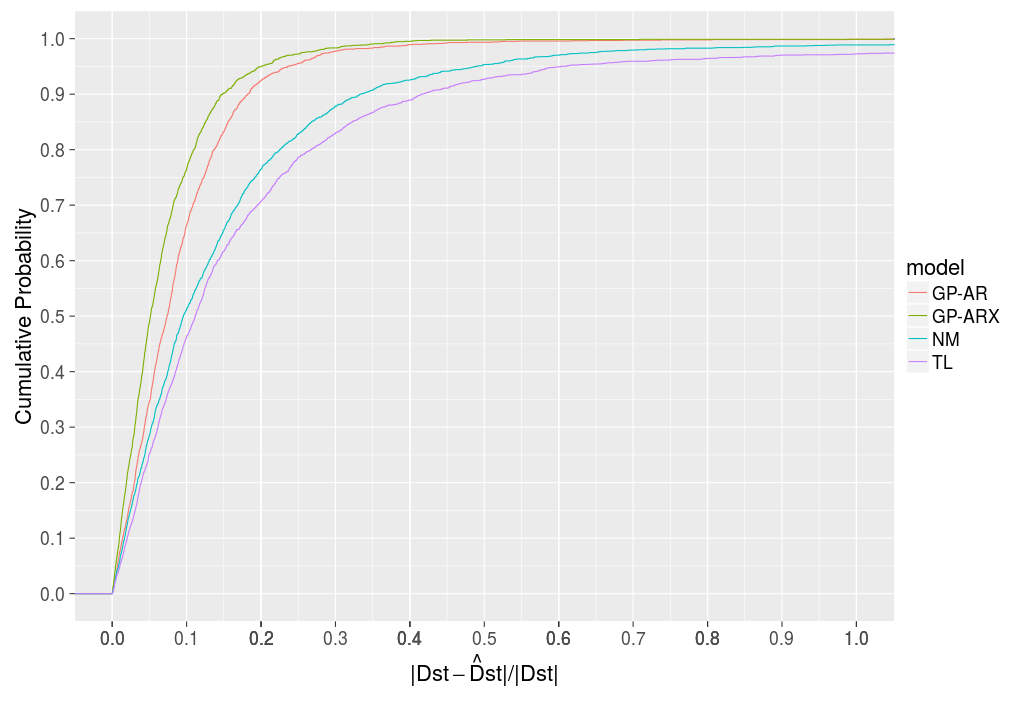
\includegraphics[width=\textwidth]{Compare_RelProb.png}
   \caption{Comparison of empirical distribution of relative errors for various models on the list of 63 storms in \citet{Ji2012}.}
   \label{fig:relprob}
\end{figure}


Apart from the metrics above, we also generate the empirical distribution of absolute relative errors $|\frac{D_{st} - \hat{D_{st}}}{D_{st}}|$ for the \emph{GP-AR}, \emph{GP-ARX}, \emph{NM} and \emph{TL} models. These empirical cumulative distributions enable us to upper bound the percentage error in $D_{st}$ prediction and attach probability estimates for said bounds.


\subsection{Models Compared}

Table \ref{table:DstModels} gives a brief enumeration of the models compared, we use the performance benchmark results published in \citet{Ji2012} and to them add results obtained from testing \emph{GP-AR}, \emph{GP-ARX} as well as the \emph{Persistence} model on the same list of storms. 

For the purpose of generating the cumulative probability plots of the model errors, we must obtain hourly predictions for all the storm events using the \emph{NARMAX} and \emph{TL} models. In the case of the \emph{NM} model, the formula outlined in \citet{balikhin:narmax} is used to generate hourly predictions. For the \emph{TL} model we use real time predictions listed on their website (\url{http://lasp.colorado.edu/home/spaceweather/}) corresponding to all the storm events. The real time predictions are at a frequency of ten minutes, hourly predictions are generated by averaging the $D_{st}$ predictions for each hour.

\begin{table}
      \caption[]{One Step Ahead $D_{st}$ prediction models compared in \citet{Ji2012}}
         \label{table:DstModels}
      
         \begin{tabular}{lll}
            \hline
            \noalign{\smallskip}
            Model  &  Reference  &  Description \\
            \noalign{\smallskip}
            \hline
            \noalign{\smallskip}
            TL & \citet{JGRA:JGRA16300} & Auto regressive model decomposable into additive terms.      \\
            NM & \citet{balikhin:narmax} & Non linear auto regressive with exogenous inputs. \\
            B & \citet{JGR:JGR10260} & Prediction of $D_{st}$ by solving ODE having injection and decay terms. \\
            W & \citet{Wang:Dst} & Obtained by modification of injection term in \citet{JGR:JGR10260}. \\
            FL & \citet{GRL:GRL11549} & Uses polarity of magnetic clouds to predict geomagnetic response.\\
            OM & \citet{JGRA:JGRA14856} & Modification of injection term in \citet{JGR:JGR10260}.\\
            \noalign{\smallskip}
            \hline
         \end{tabular}
\end{table}

\begin{figure}
   \centering
   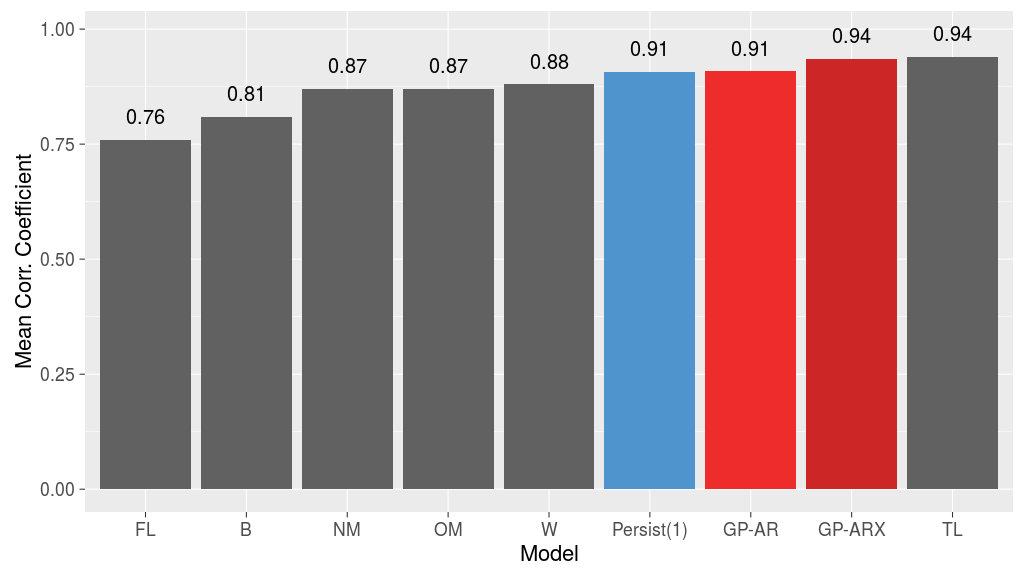
\includegraphics[width=\textwidth]{Compare_CC.png}
      \caption{Averaged Cross correlation coefficient}
         \label{fig:cc}
   \end{figure}



With respect to the \emph{TL} model one important concern must be expressed. The training of the \emph{TL} model was done on Omni data from 1996-2002 which overlaps with a large number of the storm events, therefore the experimental procedure has a strong bias towards \emph{TL} model.


\begin{figure}
   \centering
   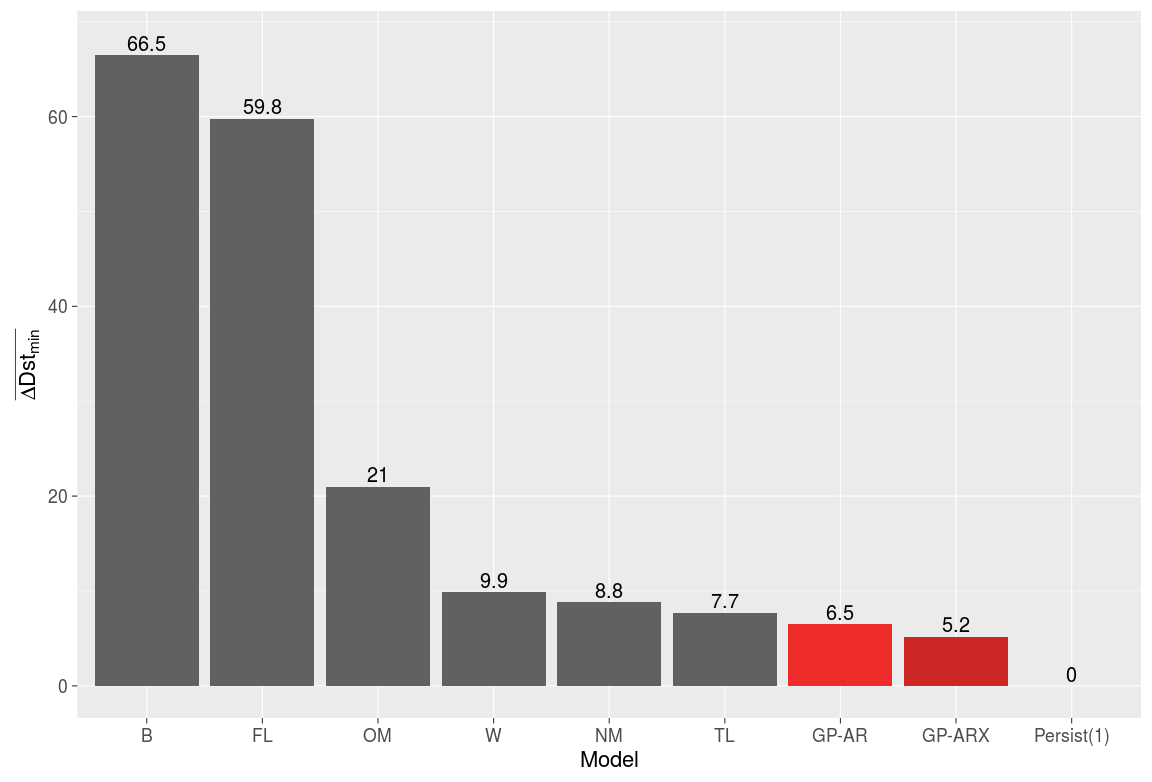
\includegraphics[width=\textwidth]{Compare_deltaDst.png}
      \caption{Averaged $\Delta Dst_{min}$}
         \label{fig:deltaDst}
   \end{figure}



\section{Results} \label{sec:res}
%%  This two-panel figure was inserted by JFW to demonstrate the subfigure and epstopdf packages
\begin{figure}
   \centering
   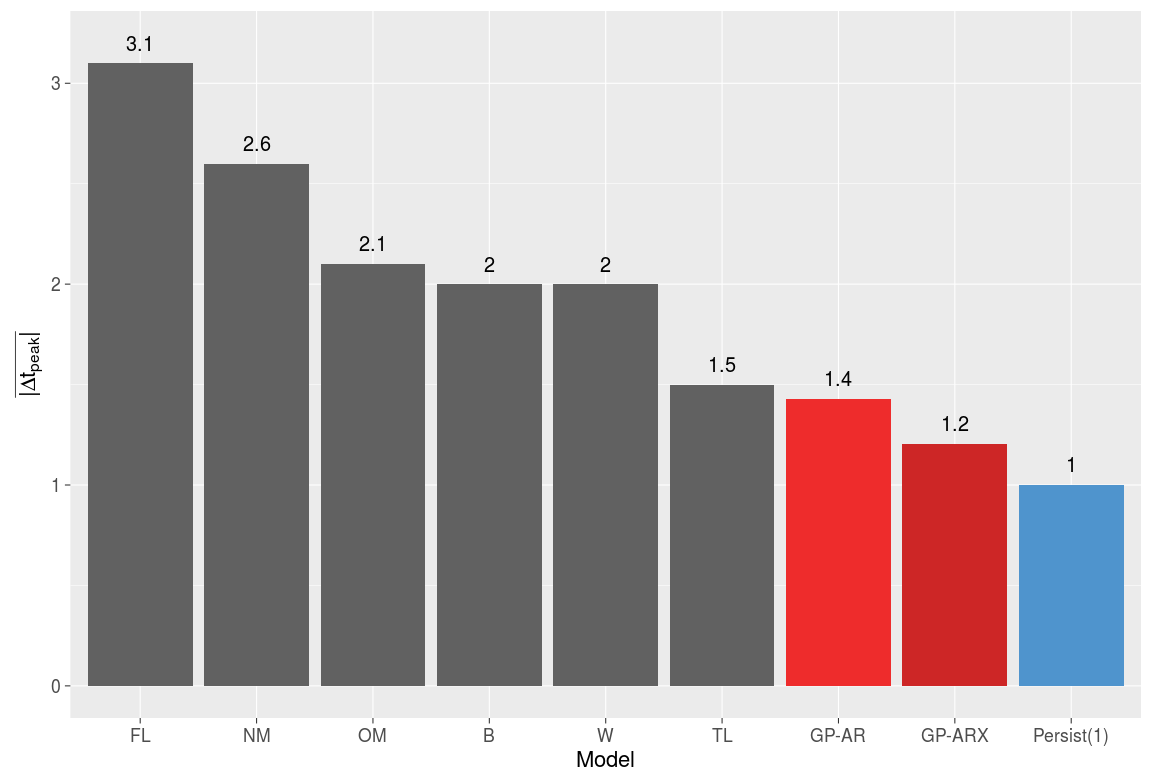
\includegraphics[width=\textwidth]{Compare_timingerr.png}
      \caption{Averaged absolute timing error}
         \label{fig:timingErr}
   \end{figure}



Figures \ref{fig:rmse}, \ref{fig:cc}, \ref{fig:deltaDst} and \ref{fig:timingErr} compare the performance of \emph{GP-AR}, \emph{GP-ARX} and the \emph{Persistence} model with the existing results of \citet{Ji2012}. Figure \ref{fig:rmse} compares the average RMSE of the models over the list of 63 storms, we can see that the \emph{GP-ARX} model gives an improvement of approximately $38\%$ in RMSE with respect to the \emph{TL} model and $60\%$ improvement with respect to the \emph{NM} model. 

Figure \ref{fig:relprob} compares the empirical distributions of absolute relative model errors across all storm events in the experiments. If one chooses a $95\%$ probability bound then it can be seen that the \emph{GP-ARX} model bounds the relative error to $20\%$ of the actual $D_{st}$ value, while in the case of the \emph{NM} model it bounds the relative error to $50\%$ of the actual $D_{st}$ value. Therefore the \emph{GP-ARX} model gives an approximate improvement of $25\%$ over the other compared models on the test data set chosen.

Figure \ref{fig:cc} shows the comparison of correlation coefficients between model predictions and actual $D_{st}$ values. From the results of \citet{Ji2012}, the \emph{TL} model gives the highest correlation coefficient of $94\%$, but that is not surprising considering the fact that there is a large overlap between the training data used to train it and storm events. This is also the case in \ref{fig:relprob} where we average predictions generated from a pre-trained instance of the \emph{TL} model. Even so the \emph{GP-ARX} model gives comparable correlation coefficient to \emph{TL} a testimony to its performance given that its training set has no overlap with the storm events.

Figure \ref{fig:deltaDst} shows how the different models compare with respect to accuracy in predicting the peak value of $D_{st}$ during storm events ($\Delta Dst_{min}$ averaged over all storms). In the context of this metric the \emph{GP-ARX} model gives a $31\%$ improvement over the \emph{TL} model and $40\%$ over the \emph{NM} model. It is trivial to note that by definition, the \emph{Persistence} model ($\hat{D_{st}}(t) = D_{st}(t-1)$) will have $\Delta Dst_{min} = 0$ for every storm instance.

Figure \ref{fig:timingErr} compares the time discrepancy of predicting the storm peak, again as observed above the \emph{Persistence} model will always have $\Delta t_{peak} = -1$, the GP-AR and GP-ARX models give better performance than the other models in terms of timing error in prediction of storm peaks. 

In figure \ref{fig:predictions} we show the OSA predictions generated by the TL, NM and GP-ARX models for one event from the list of storms in \citet{Ji2012}. This storm is interesting due to its strength ($Dst_{min} = -289 nT$) and the presence of two distinct peaks. In this particular event the GP-ARX model approximates the twin peaks as well as the onset and decay phases quite faithfully which is lacking in the NM and TL model predictions. The TL model recognises the presence of twin peaks but over estimates the second one as well as the decay phase, while the NM model is much delayed in the prediction of the initial peak and fails to approximate the time and intensity of the second peak.    

\begin{figure}
   \centering
   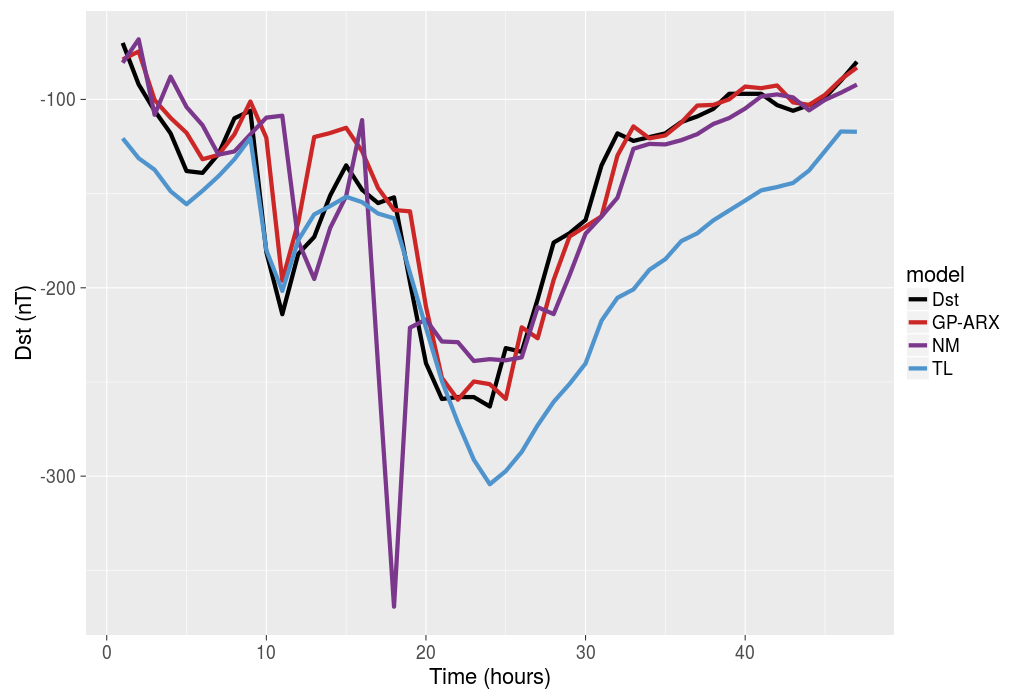
\includegraphics[width=\textwidth]{Compare_pred.png}
      \caption{Comparison of OSA predictions generated by the NM, TL and GP-ARX models for the storm event $9^{th}$ November $2004$ 11:00 UTC - $11^{th}$ November $2004$ 09:00 UTC}
         \label{fig:predictions}
   \end{figure}


\begin{comment}
\begin{enumerate}
    \item Persistence Behavior: It is clear that the \emph{persistence} behavior in the $D_{st}$ values is very strong i.e. the trivial predictive model $\hat{D_{st}}(t) = D_{st}(t-1)$ gives excellent performance. In fact it can be seen in these figures that the \emph{Persistence} model is outperforms every model compared by \citet{Ji2012} in the context of OSA prediction of $D_{st}$. Therefore any model that is proposed to tackle the OSA prediction problem for $D_{st}$ must be compared to and show visible gains over the \emph{Persistence} model.
    \item Assessment of Gaussian Process Models: The results indicate that there are many benefits to be gained by the application of Gaussian Process models for prediction of $D_{st}$. The \emph{GP-AR} and \emph{GP-ARX} not only outperform the models compared in \citet{Ji2012} but also the \emph{Persistence} model. 
\end{enumerate}
\end{comment}
  
\section{Conclusions}

We conclude this paper with three key conclusions/insights learned from our research so far.
   \begin{enumerate}
      \item \emph{Persistence} model must be central in the model evaluation process in the context of \emph{One Step Ahead} prediction of the $D_{st}$ index. It is clear that the \emph{persistence} behavior in the $D_{st}$ values is very strong i.e. the trivial predictive model $\hat{D_{st}}(t) = D_{st}(t-1)$ gives excellent performance. In fact it can be seen in \ref{sec:res} that the \emph{Persistence} model is outperforms every model compared by \citet{Ji2012} in the context of OSA prediction of $D_{st}$. Therefore any model that is proposed to tackle the OSA prediction problem for $D_{st}$ must be compared to the \emph{Persistence} model and show visible gains above it.
      
      \item \emph{Gaussian Process} AR and ARX models give encouraging benefits in OSA prediction even when compared to the \emph{Persistence} model. Leveraging the strengths of the Bayesian approach, they are able to learn robust predictors from data. 
      
      If one compares the training sets used by the models, one can appreciate that they are able to learn robust models for prediction with relatively small training and validations sets (training set contains 250 instances, while the validation set contains 432 instances) on the other hand the \emph{NM} model uses one year (8760 instances) of data to learn the formula outlined in \citet{balikhin:narmax} and the \emph{TL} model uses six years of data (52560 instances) for training. 
      
      The encouraging results of Gaussian Processes illustrate the strengths of the Bayesian approach to predictive modeling. Since the GP models generate predictive distributions for test data and not just point predictions they lend themselves to the requirements of space weather prediction very well because of the need to generate error bars on predictions.

      \item Multi-step ahead prediction should be the preferred gold standard with respect to forecasting of geomagnetic indices. Also important is the usage of more informative performance metrics for evaluating and comparing empirical predictive models.
   \end{enumerate}

\begin{acknowledgements}
      We acknowledge use of NASA/GSFC's Space Physics Data Facility's OMNIWeb (or CDAWeb or ftp) service, and OMNI data.
\end{acknowledgements}

%%    This version assumes use of bibtex with the swsc.bib file being present
%%    If your bib file has a different name you need to change the following line

\bibliography{swsc}

\end{linenumbers}

\end{document}

%%    If you wish to include your bibliography items in your tex file 
%%    using {thebibliography} as shown below you must out-comment the 
%%    three lines above (insert % at the start of each line) 

\begin{thebibliography}{}

   \bibitem[Baker(1966)]{baker} Baker, N., Solar Evolution,
      in Stellar Evolution, ed.\ R. F. Stein and A. G. W. Cameron,
      Plenum, New York, 333, 1966.

   \bibitem[Balluch(1988)]{balluch} Balluch, M., A paper on something, 
      {\it Astron. Astrophys}, {\bf 200}, 58-63, 1988.

   \bibitem[Cox(1980)]{cox} Cox, J. P.,
      Theory of Stellar Pulsation,
      Princeton University Press, Princeton, 1980.

   \bibitem[Cox and Stewart(1969)]{cox69} Cox, A. N., and J. N. Stewart,
      Academia Nauk, {\it Scientific Information}, {\bf 15}, 1-11, 1969.

   \bibitem[Dumm and Kopf(2014)]{dummkopf} Dumm, Z., and Z. Kopf, A new self-inconsistent 
      core stability model, 
      {\it J. Space Weather Space Clim.}, {\bf 4}, A00, 2014, DOI: 10.1051/swsc/2014000,
      \url{http://dx.doi.org/10.1051/swsc/2014000}.

   \bibitem[Fool(2012)]{fool} Fool, X. Y., All earlier results are wrong, 
      {\it J. Space Weather Space Clim.}, {\bf 2}, A00, 2012, DOI: 10.1051/swsc/2012000,
      \url{http://dx.doi.org/10.1051/swsc/2012000}.

   \bibitem[Fou(2013)]{fou} Fou, Y. X., No earlier results were right, 
      {\it J. Space Weather Space Clim.}, {\bf 3}, A00, 2013, DOI: 10.1051/swsc/2013000,
      \url{http://dx.doi.org/10.1051/swsc/2013000}.

   \bibitem[Kr\"ugel et al.(1971)]{krugel71} Kr\"ugel, A. H., A. F. Davidsen, D. Tytler, and G. A. Kriss, 
      Summary of Project Achievements, Technical Report 08-11, 
      Fake Company, Nowherecity, Nowhereland, 1971.

   \bibitem[Mizuno(1980)]{mizuno} Mizuno, H., A further step backward in scientific understanding, 
      {\it Prog. Theor. Phys.}, {\bf 64}, 544-545, 1980.
   
   \bibitem[Tscharnuter(1987)]{tscharnuter} Tscharnuter, W. M., Who knows about astronomy?, 
      {\it Astron. Astrophys}, {\bf 188}, 55-57, 1987.

   \bibitem[Yorke(1980a)]{yorke80a} Yorke, H. W., A paper on nothing, 
      {\it Astron. Astrophys}, {\bf 86}, 286, 1980a.

   \bibitem[Yorke(1980b)]{yorke80b} Yorke, H. W., A paper on everything, 
      {\it Astron. Astrophys}, {\bf 86}, 291, 1980b.

\end{thebibliography}

\end{linenumbers}

\end{document}

%%%%%%%%%%%%%%%%%%%%%%%%%%%%%%%%%%%%%%%%%%%%%%%%%%%%%%%%%%%%%%%%%%%%%%%%%%%
%%
%%   Below are examples of how to use particular document layout features
%%
%%%%%%%%%%%%%%%%%%%%%%%%%%%%%%%%%%%%%%%%%%%%%%%%%%%%%%%%%%%%%%%%%%%%%%%%%%%
%%  Examples for figures using graphicx
%%  A guide "Using Imported Graphics in LaTeX2e"  (Keith Reckdahl)
%%  is available on a lot of LaTeX public servers or ctan mirrors.
%%  The file is : epslatex.pdf 
%%%%%%%%%%%%%%%%%%%%%%%%%%%%%%%%%%%%%%%%%%%%%%%%%%%%%%%%%%%%%%%%%%%%%%%%%%%

%_____________________________________________________________
%                 A figure as large as the width of the column
%-------------------------------------------------------------
   \begin{figure}
   \centering
   \includegraphics[width=\textwidth]{empty.eps}
      \caption{Vibrational stability equation of state
               $S_{\mathrm{vib}}(\lg e, \lg \rho)$.
               $>0$ means vibrational stability.
              }
         \label{FigVibStab}
   \end{figure}
%
%_____________________________________________________________
%                                    One column rotated figure
%-------------------------------------------------------------
   \begin{figure}
   \centering
   \includegraphics[angle=-90,width=3cm]{empty.eps}
      \caption{Vibrational stability equation of state
               $S_{\mathrm{vib}}(\lg e, \lg \rho)$.
               $>0$ means vibrational stability.
              }
         \label{FigVibStab}
   \end{figure}
%
%_____________________________________________________________
%                        Figure with caption on the right side 
%-------------------------------------------------------------
   \begin{figure}
   \centering
   \includegraphics[width=3cm]{empty.eps}
      \caption{Vibrational stability equation of state
               $S_{\mathrm{vib}}(\lg e, \lg \rho)$.
               $>0$ means vibrational stability.
              }
         \label{FigVibStab}
   \end{figure}
%
%_____________________________________________________________
%
%_____________________________________________________________
%                                Figure with a new BoundingBox 
%-------------------------------------------------------------
   \begin{figure}
   \centering
   \includegraphics[bb=10 20 100 300,width=3cm,clip]{empty.eps}
      \caption{Vibrational stability equation of state
               $S_{\mathrm{vib}}(\lg e, \lg \rho)$.
               $>0$ means vibrational stability.
              }
         \label{FigVibStab}
   \end{figure}
%
%_____________________________________________________________
%
%_____________________________________________________________
%                                      The "resizebox" command 
%-------------------------------------------------------------
   \begin{figure}
   \resizebox{\textwidth}{!}
            {\includegraphics[bb=10 20 100 300,clip]{empty.eps}
      \caption{Vibrational stability equation of state
               $S_{\mathrm{vib}}(\lg e, \lg \rho)$.
               $>0$ means vibrational stability.
              }
         \label{FigVibStab}
   \end{figure}
%
%______________________________________________________________
%
%_____________________________________________________________
%                                             Simple A&A Table
%_____________________________________________________________
%
\begin{table}
\caption{Nonlinear Model Results}             % title of Table
\label{table:1}      % is used to refer this table in the text
\centering                          % used for centering table
\begin{tabular}{c c c c}        % centered columns (4 columns)
\hline\hline                 % inserts double horizontal lines
HJD & $E$ & Method\#2 & Method\#3 \\    % table heading 
\hline                        % inserts single horizontal line
   1 & 50 & $-837$ & 970 \\      % inserting body of the table
   2 & 47 & 877    & 230 \\
   3 & 31 & 25     & 415 \\
   4 & 35 & 144    & 2356 \\
   5 & 45 & 300    & 556 \\ 
\hline                                   %inserts single line
\end{tabular}
\end{table}
%
%_____________________________________________________________
%                                             Two column Table 
%_____________________________________________________________
%
\begin{table*}
\caption{Nonlinear Model Results}             
\label{table:1}      
\centering          
\begin{tabular}{c c c c l l l }     % 7 columns 
\hline\hline       
                      % To combine 4 columns into a single one 
HJD & $E$ & Method\#2 & \multicolumn{4}{c}{Method\#3}\\ 
\hline                    
   1 & 50 & $-837$ & 970 & 65 & 67 & 78\\  
   2 & 47 & 877    & 230 & 567& 55 & 78\\
   3 & 31 & 25     & 415 & 567& 55 & 78\\
   4 & 35 & 144    & 2356& 567& 55 & 78 \\
   5 & 45 & 300    & 556 & 567& 55 & 78\\
\hline                  
\end{tabular}
\end{table*}
%
%-------------------------------------------------------------
%                                          Table with notes 
%-------------------------------------------------------------
%
% A single note
\begin{table}[h]
\caption{\label{t7}Spectral types and photometry for stars in the
  region.}
\centering
\begin{tabular}{lccc}
\hline\hline
Star&Spectral type&RA(J2000)&Dec(J2000)\\
\hline
69           &B1\,V     &09 15 54.046 & $-$50 00 26.67\\
49           &B0.7\,V   &*09 15 54.570& $-$50 00 03.90\\
LS~1267~(86) &O8\,V     &09 15 52.787&11.07\\
24.6         &7.58      &1.37 &0.20\\
\hline
LS~1262      &B0\,V     &09 15 05.17&11.17\\
MO 2-119     &B0.5\,V   &09 15 33.7 &11.74\\
LS~1269      &O8.5\,V   &09 15 56.60&10.85\\
\hline
\end{tabular}
\tablefoot{ The top panel shows likely members of Pismis~11. The second
panel contains likely members of Alicante~5. The bottom panel
displays stars outside the clusters.}
\end{table}
%
% More notes
%
\begin{table}[h]
\caption{\label{t7}Spectral types and photometry for stars in the
  region.}
\centering
\begin{tabular}{lccc}
\hline\hline
Star&Spectral type&RA(J2000)&Dec(J2000)\\
\hline
69           &B1\,V     &09 15 54.046 & $-$50 00 26.67\\
49           &B0.7\,V   &*09 15 54.570& $-$50 00 03.90\\
LS~1267~(86) &O8\,V     &09 15 52.787&11.07\tablefootmark{a}\\
24.6         &7.58\tablefootmark{1}&1.37\tablefootmark{a}   &0.20\tablefootmark{a}\\
\hline
LS~1262      &B0\,V     &09 15 05.17&11.17\tablefootmark{b}\\
MO 2-119     &B0.5\,V   &09 15 33.7 &11.74\tablefootmark{c}\\
LS~1269      &O8.5\,V   &09 15 56.60&10.85\tablefootmark{d}\\
\hline
\end{tabular}
\tablefoot{ The top panel shows likely members of Pismis~11. The second
panel contains likely members of Alicante~5. The bottom panel
displays stars outside the clusters.\\
\tablefoottext{a}{Photometry for MF13, LS~1267 and HD~80077 from
Dupont et al.}
\tablefoottext{b}{Photometry for LS~1262, LS~1269 from
Durand et al.}
\tablefoottext{c}{Photometry for MO2-119 from
Mathieu et al.}
}
\end{table}
%
%-------------------------------------------------------------
%                                       Table with references 
%-------------------------------------------------------------
%
\begin{table*}[h]
 \caption[]{\label{nearbylistaa2}List of nearby SNe used in this work.}
\begin{tabular}{lccc}
 \hline \hline
  SN name &
  Epoch &
 Bands &
  References \\
 &
  (with respect to $B$ maximum) &
 &
 \\ \hline
1981B   & 0 & {\it UBV} & 1\\
1986G   &  $-$3, $-$1, 0, 1, 2 & {\it BV}  & 2\\
1989B   & $-$5, $-$1, 0, 3, 5 & {\it UBVRI}  & 3, 4\\
1990N   & 2, 7 & {\it UBVRI}  & 5\\
1991M   & 3 & {\it VRI}  & 6\\
\hline
\noalign{\smallskip}
\multicolumn{4}{c}{ SNe 91bg-like} \\
\noalign{\smallskip}
\hline
1991bg   & 1, 2 & {\it BVRI}  & 7\\
1999by   & $-$5, $-$4, $-$3, 3, 4, 5 & {\it UBVRI}  & 8\\
\hline
\noalign{\smallskip}
\multicolumn{4}{c}{ SNe 91T-like} \\
\noalign{\smallskip}
\hline
1991T   & $-$3, 0 & {\it UBVRI}  &  9, 10\\
2000cx  & $-$3, $-$2, 0, 1, 5 & {\it UBVRI}  & 11\\ %
\hline
\end{tabular}
\tablebib{(1)~\citet{branch83};
(2) \citet{phillips87}; (3) \citet{barbon90}; (4) \citet{wells94};
(5) \citet{mazzali93}; (6) \citet{gomez98}; (7) \citet{kirshner93};
(8) \citet{patat96}; (9) \citet{salvo01}; (10) \citet{branch03};
(11) \citet{jha99}.
}
\end{table}
%_____________________________________________________________
%                                 A rotated Table in landscape  
%  In the preamble, use:   \usepackage{lscape}
%-------------------------------------------------------------
\begin{landscape}
\begin{table*}
\caption{Summary for ISOCAM sources with mid-IR excess 
(YSO candidates).}\label{YSOtable}
\centering
\begin{tabular}{crrlcl} 
\hline\hline             
ISO-L1551 & $F_{6.7}$~[mJy] & $\alpha_{6.7-14.3}$ 
& YSO type$^{d}$ & Status & Comments\\
\hline
  \multicolumn{6}{c}{\it New YSO candidates}\\ % To combine 6 columns into a single one
\hline
  1 & 1.56 $\pm$ 0.47 & --    & Class II$^{c}$ & New & Mid\\
  2 & 0.79:           & 0.97: & Class II ?     & New & \\
  3 & 4.95 $\pm$ 0.68 & 3.18  & Class II / III & New & \\
  5 & 1.44 $\pm$ 0.33 & 1.88  & Class II       & New & \\
\hline
  \multicolumn{6}{c}{\it Previously known YSOs} \\
\hline
  61 & 0.89 $\pm$ 0.58 & 1.77 & Class I & \object{HH 30} & Circumstellar disk\\
  96 & 38.34 $\pm$ 0.71 & 37.5& Class II& MHO 5          & Spectral type\\
\hline
\end{tabular}
\end{table*}
\end{landscape}
%
%_____________________________________________________________
%                              Table longer than a single page  
%  In the preamble, use:              \usepackage{longtable}
%-------------------------------------------------------------
%          All long tables have to be placed at the end, after 
%                                        \end{thebibliography}
%
% In the text, at the place where the large table should appear
% add the command:
\addtocounter{table}{1}
% Tables counters will be well numbered.
%
\end{thebibliography}
% If table 2
\longtab{2}{
\begin{longtable}{lllrrr}
\caption{\label{kstars} Sample stars with absolute magnitude}\\
\hline\hline
Catalogue& $M_{V}$ & Spectral & Distance & Mode & Count Rate \\
\hline
\endfirsthead
\caption{continued.}\\
\hline\hline
Catalogue& $M_{V}$ & Spectral & Distance & Mode & Count Rate \\
\hline
\endhead
\hline
\endfoot
%%
Gl 33    & 6.37 & K2 V & 7.46 & S & 0.043170\\
Gl 66AB  & 6.26 & K2 V & 8.15 & S & 0.260478\\
Gl 68    & 5.87 & K1 V & 7.47 & P & 0.026610\\
         &      &      &      & H & 0.008686\\
Gl 86 
\footnote{Source not included in the HRI catalog. See Sect.~5.4.2 for details.}
         & 5.92 & K0 V & 10.91& S & 0.058230\\
\end{longtable}
}% End \longtab
%
%_____________________________________________________________
%                              Table longer than a single page
%                                             and in landscape 
%  In the preamble, use:       \usepackage{longtable,lscape}
%-------------------------------------------------------------
%          All long tables have to be placed at the end, after
%                                        \end{thebibliography}
%
% In the text, at the place where the large table should appear
% add the command:                        
\addtocounter{table}{1} 
% Tables counters will be well numbered.
%
\end{thebibliography}
% If table 2
\longtabL{2}{
\begin{landscape}
\begin{longtable}{lllrrr}
\caption{\label{kstars} Sample stars with absolute magnitude}\\
\hline\hline
Catalogue& $M_{V}$ & Spectral & Distance & Mode & Count Rate \\
\hline
\endfirsthead
\caption{continued.}\\
\hline\hline
Catalogue& $M_{V}$ & Spectral & Distance & Mode & Count Rate \\
\hline
\endhead
\hline
\endfoot
%%
Gl 33    & 6.37 & K2 V & 7.46 & S & 0.043170\\
Gl 66AB  & 6.26 & K2 V & 8.15 & S & 0.260478\\
Gl 68    & 5.87 & K1 V & 7.47 & P & 0.026610\\
         &      &      &      & H & 0.008686\\
Gl 86
\footnote{Source not included in the HRI catalog. See Sect.~5.4.2 for details.}
         & 5.92 & K0 V & 10.91& S & 0.058230\\
\end{longtable}
\end{landscape}
}% End \longtabL
%
% Online Material
%_____________________________________________________________
%        Online appendices have to be placed at the end, after
%                                        \end{thebibliography}
%-------------------------------------------------------------
\end{thebibliography}

\Online

\begin{appendix} %First online appendix
\section{Background galaxy number counts and shear noise-levels}
Because the optical images used in this analysis...

\begin{figure*}
\centering
\includegraphics[width=16.4cm,clip]{1787f24.ps}
\caption{Plotted above...}
\label{appfig}
\end{figure*}

Because the optical images...
\end{appendix}

\begin{appendix} %Second online appendix
These studies, however, have faced...
\end{appendix}

\end{document}
%
%_____________________________________________________________
%        Some tables or figures are in the printed version and
%                      some are only in the electronic version
%-------------------------------------------------------------
%
% Leave all the tables or figures in the text, at their right place 
% and use the commands \onlfig{}{} and \onltab{}{}. These elements
% will be automatically placed at the end, in the section
% Online material.

\documentclass{swsc}
...
\begin{document}
text of the paper...
\begin{figure*}%f1
\includegraphics[width=10.9cm]{1787f01.eps}
\caption{Shown in greyscale is a...}
\label{cl12301}}
\end{figure*}
...
from the intrinsic ellipticity distribution.
% Figure 2 available electronically only
\onlfig{2}{
\begin{figure*}%f2
\includegraphics[width=11.6cm]{1787f02.eps}
\caption {Shown in greyscale...}
\label{cl1018}
\end{figure*}
}

% Figure 3 available electronically only
\onlfig{3}{
\begin{figure*}%f3
\includegraphics[width=11.2cm]{1787f03.eps}
\caption{Shown in panels...}
\label{cl1059}
\end{figure*}
}

\begin{figure*}%f4
\includegraphics[width=10.9cm]{1787f04.eps}
\caption{Shown in greyscale is...}
\label{cl1232}}
\end{figure*}

\begin{table}%t1
\caption{Complexes characterisation.}\label{starbursts}
\centering
\begin{tabular}{lccc}
\hline \hline
Complex & $F_{60}$ & 8.6 &  No. of  \\
...
\hline
\end{tabular}
\end{table}
The second method produces...

% Figure 5 available electronically only
\onlfig{5}{
\begin{figure*}%f5
\includegraphics[width=11.2cm]{1787f05.eps}
\caption{Shown in panels...}
\label{cl1238}}
\end{figure*}
}

As can be seen, in general the deeper...
% Table 2 available electronically only
\onltab{2}{
\begin{table*}%t2
\caption{List of the LMC stellar complexes...}\label{Properties}
\centering
\begin{tabular}{lccccccccc}
\hline  \hline
Stellar & RA & Dec & ...
...
\hline
\end{tabular}
\end{table*}
}

% Table 3 available electronically only
\onltab{3}{
\begin{table*}%t3
\caption{List of the derived...}\label{IrasFluxes}
\centering
\begin{tabular}{lcccccccccc}
\hline \hline
Stellar & $f12$ & $L12$ &...
...
\hline
\end{tabular}
\end{table*}
}
%
%-------------------------------------------------------------
%     For the online material, table longer than a single page
%                 In the preamble, use: \usepackage{longtable}
%       or for landscape option: \usepackage{longtable,lscape}
%-------------------------------------------------------------
\documentclass{swsc}
\usepackage[varg]{txfonts}
\usepackage{graphicx}
\usepackage{longtable}

\begin{document}
text of the paper
% Table will be print automatically at the end, in the section Online material.
\onllongtab{3}{
\begin{longtable}{lrcrrrrrrrrl}
\caption{Line data and abundances ...}\\
\hline
\hline
Def & mol & Ion & $\lambda$ & $\chi$ & $\log gf$ & N & e &  rad & $\delta$ & $\delta$ 
red & References \\
\hline
\endfirsthead
\caption{Continued.} \\
\hline
Def & mol & Ion & $\lambda$ & $\chi$ & $\log gf$ & B & C &  rad & $\delta$ & $\delta$ 
red & References \\
\hline
\endhead
\hline
\endfoot
\hline
\endlastfoot
A & CH & 1 &3638 & 0.002 & $-$2.551 &  &  &  & $-$150 & 150 &  Jorgensen et al. (1996) \\                    
\end{longtable}
}% End onllongtab

% Or for landscape, large table:

\onllongtabL{3}{
\begin{landscape}
\begin{longtable}{lrcrrrrrrrrl}
...
\end{longtable}
\end{landscape}
}% End onllongtabL

